% !Mode:: "TeX:UTF-8"
\chapter{国内外研究现状}

\section{博物馆中的信息导览方式}
近年研究表明，相较于博物馆中常见的固定顺序的文本、音频或说明牌呈现，对话式、可交互的讲述方式更有助于激发观众参与。
在虚拟博物馆与沉浸式文化遗产体验中，引入支持自然语言提问的对话式讲述者，能够显著提升沉浸感、存在感与整体体验评价\cite{cannavo2024,olaz2022,okanovic2022}。在非沉浸式数字导览与线上文化遗产平台中，对话式机制同样表现出相对于静态页面的优势，用户研究表明，集成自由问答与上下文相关问题建议的文化遗产网站，在可用性与信息探索体验上显著优于仅依赖静态网页浏览的形式，尤其能够支持用户围绕自身兴趣进行更深入的内容探索\cite{cossatin2025}。围绕博物馆聊天机器人的研究进一步指出，访客普遍期望通过对话进行学习与探索，对话式界面在信息可达性与学习动机方面具有明显优势\cite{duguleana2020,spiliotopoulos2020,varitimiadis2021}。从文化遗产叙事与长期参与的角度来看，互动式叙事同样被证明优于线性或静态呈现方式，互动纪录片、交互式投影映射与多路径数字叙事装置通过允许观众选择内容与触发叙事进程，在理解深度、记忆保持与持续参与方面表现更优\cite{podara2021,nikolakopoulou2022}。在文化遗产教育场景中，结合 AI 的情境化多线叙事与实时问答机制，也被证实能够显著提升知识掌握与文化认同，相较于单向讲解具有更高的学习成效\cite{yu2025heritage}。
在国内实践中，国家博物馆“蒋雯雯数字人”属于典型的脚本化数字人导览案例，如图\ref{fig:scripted-museum-digital-human}所示：其展示形态以预设讲解动画为主，能够完成内容播报与形象呈现，但缺少面向观众问题的实时交互机制与连续对话能力。该类系统在传播一致性与展示稳定性方面具有优势，但在开放参观场景中难以根据观众提问、关注点变化与参观阶段进行动态引导，因而更接近可视化讲解而非可交互导览。

\begin{figure}[htbp]
    \centering
    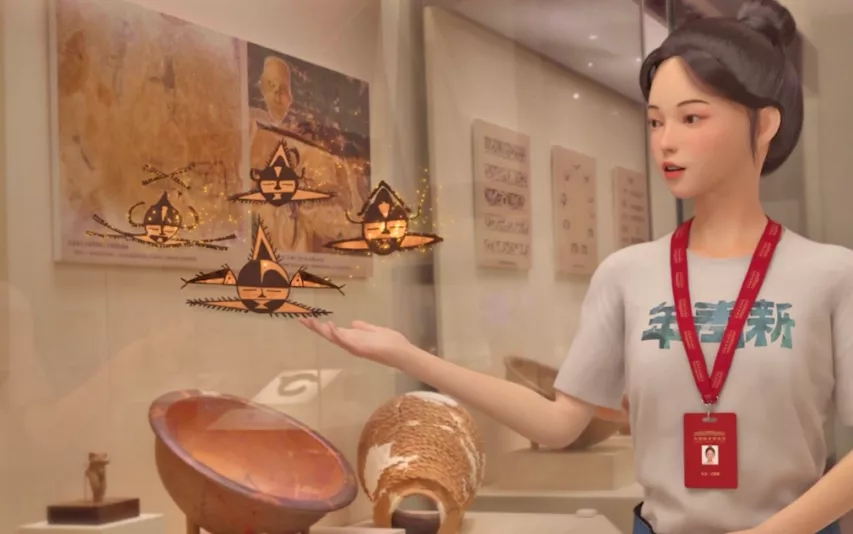
\includegraphics[width=\textwidth]{figure/figs/脚本化数字人.png}
    \caption{脚本化博物馆数字人（来源：国家博物馆官网）}
    \label{fig:scripted-museum-digital-human}
\end{figure}

综上所述，尽管当今多数博物馆使用是固定顺序的文本展示，\textbf{对话式、可交互的讲述机制更符合博物馆与文化学习场景中观众的理解方式与参与需求}。

\section{博物馆导览中的学习情境理解}
博物馆学习研究普遍认为，学习发生在观众的具体参观过程中，由空间、对象与个体动机共同构成的情境中逐步展开。
Falk 与 Dierking 提出的情境学习模型指出，博物馆体验由物理情境、社会文化情境与个人情境相互交织而成，学习意义正是在这种多维情境的作用下被建构\cite{falk2016}。多项研究表明，在博物馆与文化遗产学习场景中，学习情境通常由三个核心要素共同构成：访客所处的空间位置、当前关注或互动的展品对象，以及访客当下的目标、问题或参观动机。
Luo、Doucé 与 Nys 在对多感官博物馆体验的综述中指出，参观者的注意力与意义建构受到其所在空间、正在互动的具体展品以及个人目标与动机的共同影响，这些要素共同构成可用于引导设计的整体情境框架，而情境模型的价值在于为情境化、个性化的引导策略提供依据，如图\ref{fig:guidance-context-model}所示\cite{luo2024}。

\begin{figure}[htbp]
    \centering
    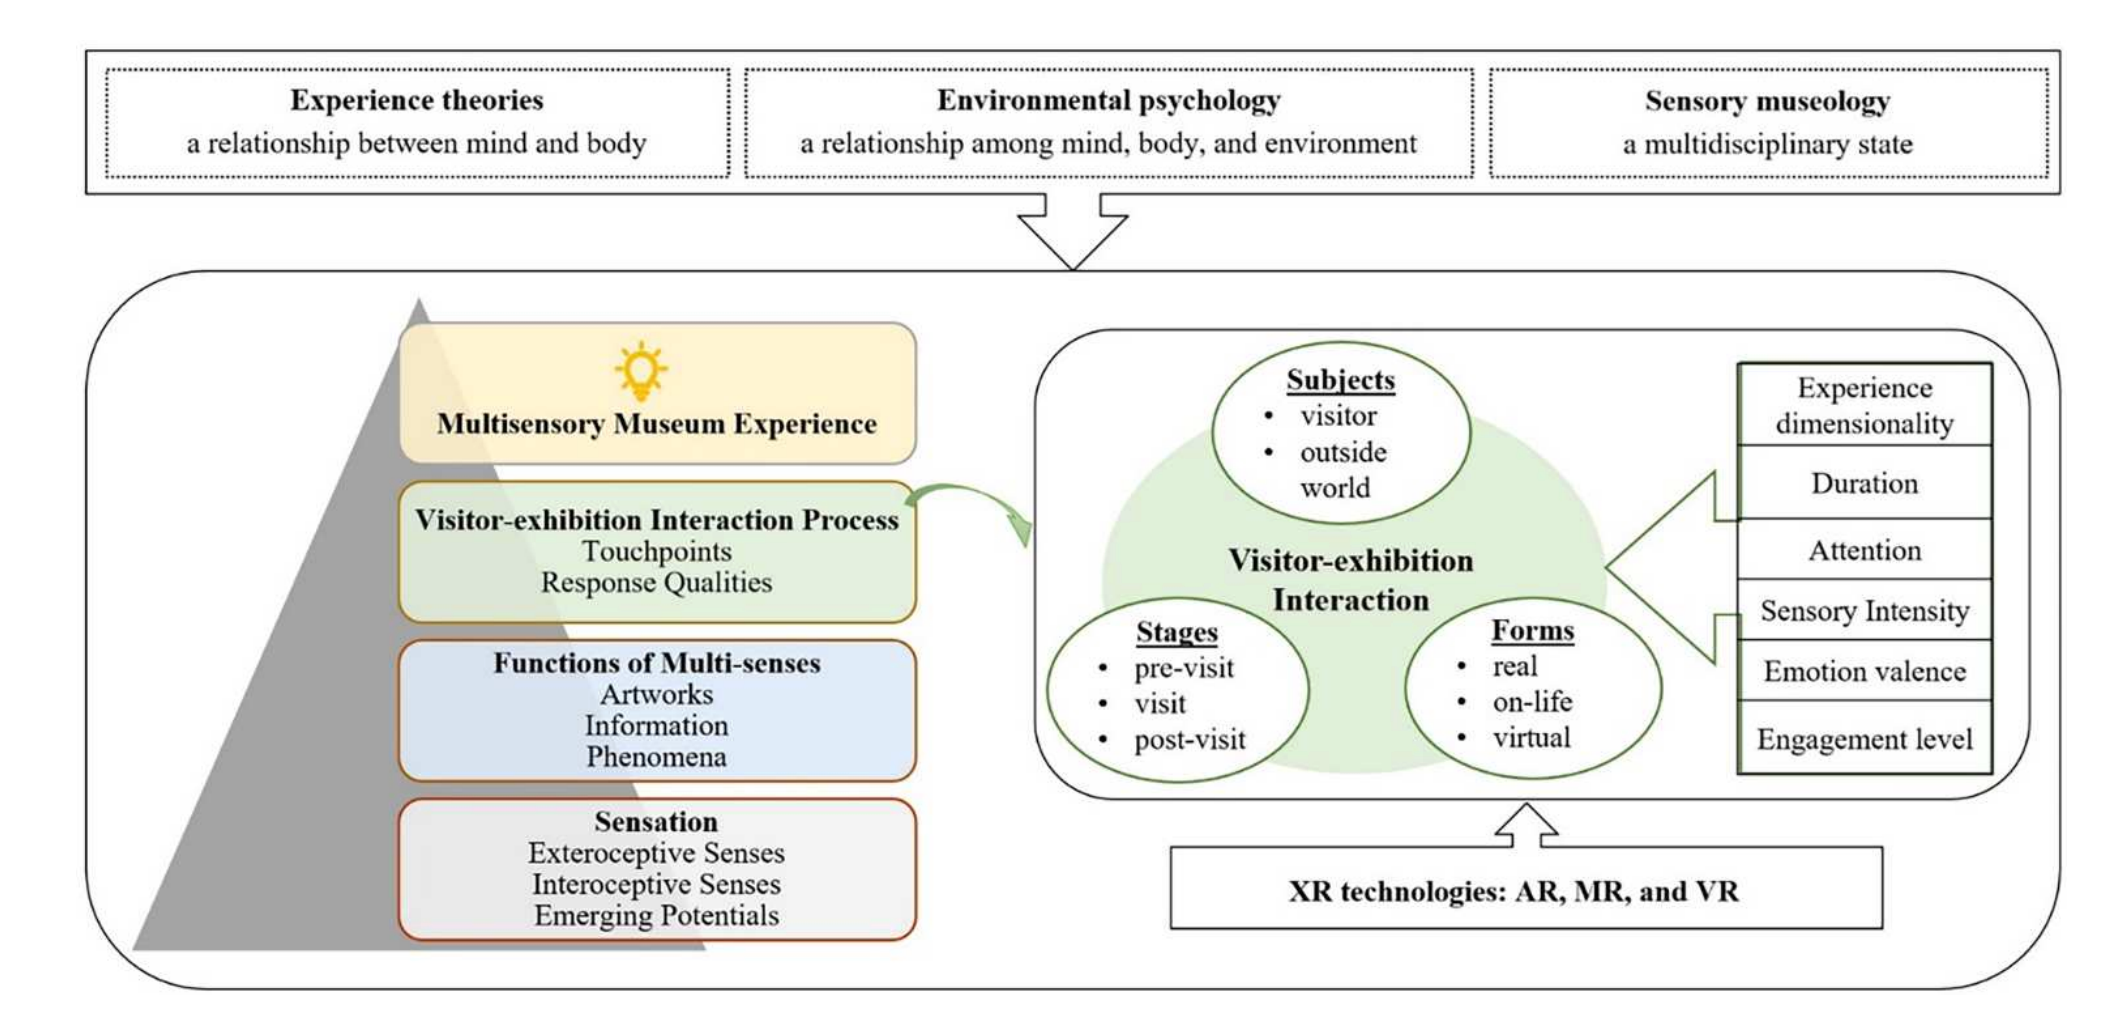
\includegraphics[width=\textwidth]{figure/figs/引导情境模型.png}
    \caption{博物馆研究中的导览情境建模（图片来自文献\cite{luo2024}）}
    \label{fig:guidance-context-model}
\end{figure}

在虚拟与数字博物馆研究中，这一观点得到进一步实证支持。Hulusić 等将虚拟文化遗产应用视为情境化学习环境，指出有效的学习支持依赖系统对用户所在空间位置、当前交互展品以及所参与任务或活动的感知，与仅推送多媒体信息的系统相比，将讲解内容与用户所处位置和关注对象绑定的情境化设计，能够显著提升参与度与理解深度，而这一过程并不需要对学习者进行精细的认知诊断\cite{hulusic2023,yu2025heritage}。
实体博物馆中的实证研究同样显示，空间情境对学习过程具有关键影响：Nofal 等通过比较不同空间配置下的任务表现发现，学习活动是否与具体文物及其所在空间紧密绑定，会显著影响知识获取顺序、参与程度与协作质量\cite{nofal2020}；Chin、Chang 与 Wang 的混合现实研究亦表明，通过位置感知将数字信息叠加至学生当前观看的展品附近，相较于非情境化的移动学习系统，能够在不增加额外认知负荷的前提下显著提升理解与保持效果\cite{chin2023}。
此外，访客的参观意图与即时问题被认为是学习情境的重要组成部分。Li 从访客体验视角指出，博物馆参观者的知识探索动机与具体展品和参观路径相互作用，影响参与方式与意义建构\cite{li2024}；相关研究进一步表明，当导览系统能够基于访客当前任务进度或问题提供针对性的提示时，学习成效、动机与沉浸体验均显著提升\cite{liu2025}。在科学博物馆情境中，Nygren、Price 与 Jha 的研究同样显示，引导者只需把握学习者正在关注的对象部分及其通过语言或行动显现的意图，即可有效调整引导方式并促进意义建构，而无需对学习者的认知状态进行显式推断\cite{nygren2023}。
综上所述，近年的博物馆与非正规学习研究普遍表明，\textbf{学习情境可被理解为由访客所处位置、当前关注对象以及当下意图或问题共同构成的整体结构，对这一情境及其互动历史的感知，有助于系统在合适的时间、围绕合适的对象、以合适的方式提供学习引导}。

\section{数字人导览交互感知与多模态表达}
认知科学与神经科学研究表明，人类对知识与概念的理解并非仅依赖抽象符号或语言处理，而是通过感知、动作与情绪等多种系统的协同参与完成。基于 fMRI 的研究发现，语义概念在大脑中的表征会同时激活与之相关的视觉、动作与情绪区域，而非仅限于语言中枢\cite{barsalou2008,huth2016}；具身认知理论进一步指出，概念理解依赖感知—运动模拟机制，认知过程本质上是对经验的再激活\cite{mitchell2008}。相关综述亦表明，具身与多模态呈现能够调动更多认知通道参与概念加工，从而提升理解深度与长期记忆保持\cite{zeman2023,vanderheiden2022}。在人机交互与虚拟现实研究中，这一理论基础已获得充分实证支持。研究表明，具身虚拟代理通过注视、手势、姿态与语音韵律等多模态行为，能够有效传递交互意图，增强社会存在感，并显著提升用户的参与度与沉浸体验；相较于纯文本或语音系统，具身代理更容易被用户感知为具有意向性的社会主体，从而在引导、解释与协作任务中发挥积极作用\cite{bailenson2008,demelo2014,kraemer2015}。进一步的研究指出，多模态行为不仅在“是否具身”的层面产生影响，其具体表达方式还会被用户整合为对代理人格化的整体感知。通过语言风格、对话节奏、身体姿态和表情等线索，用户会自然形成外向/内向、亲和/权威等人格判断，而这些人格化线索会显著影响信任、好感度与互动投入程度；即使在任务内容不变的情况下，仅通过操控对话风格或非语言行为，也能够系统性地改变用户对代理的社会评价与引导接受度\cite{lester2015,roussou2018,crowley2001,kong2020,lv2017,huang2011}。

\begin{figure}[htbp]
    \centering
    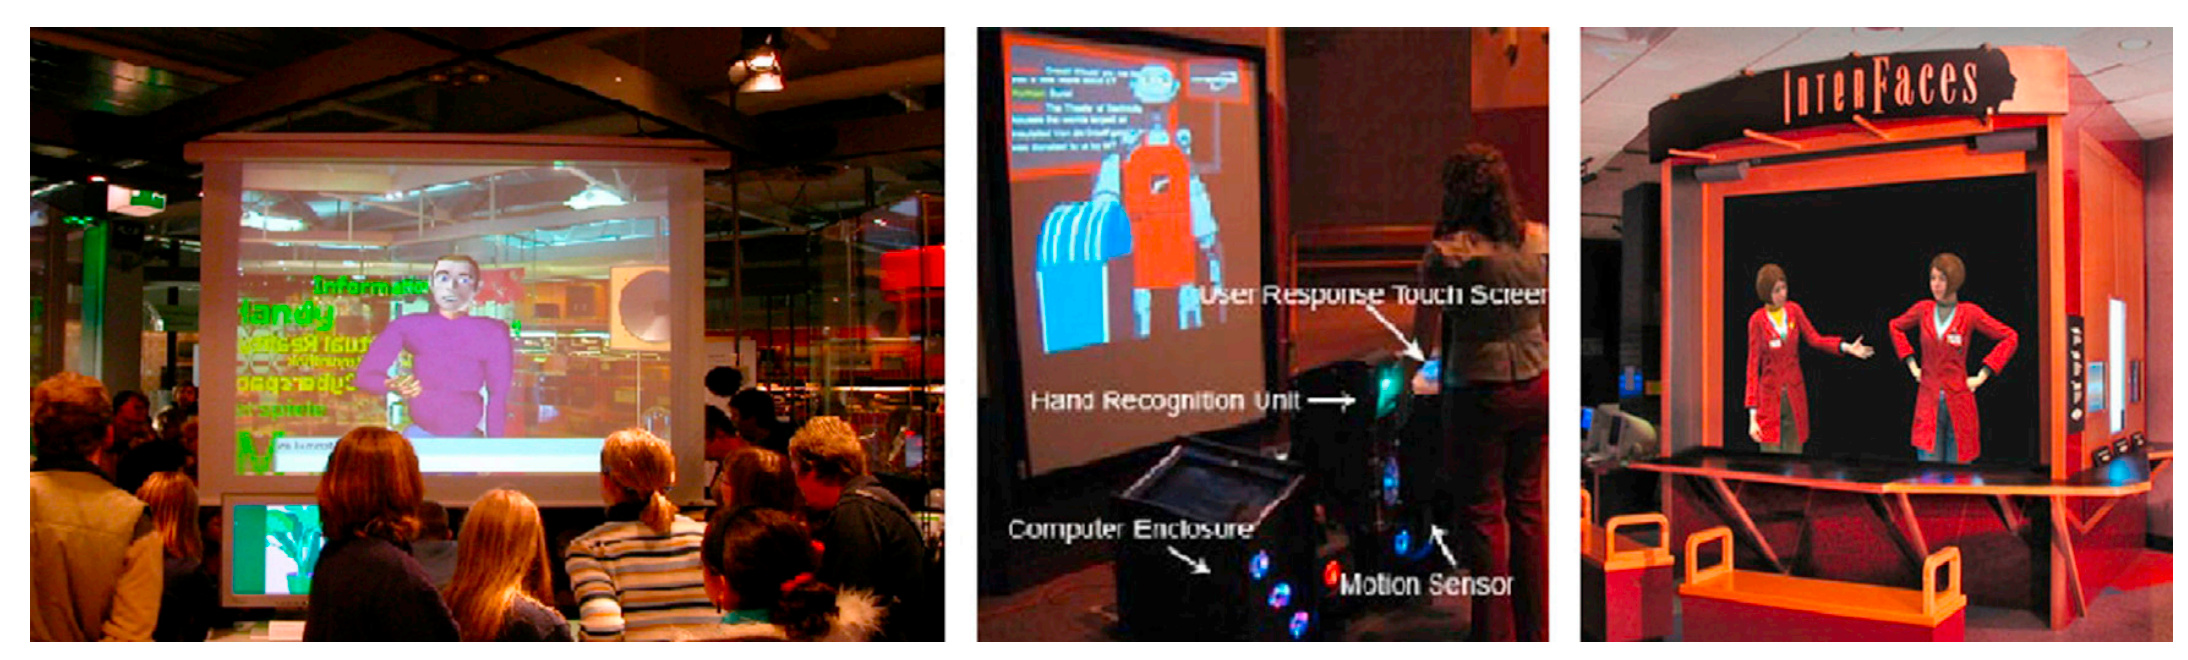
\includegraphics[width=\textwidth]{figure/figs/博物馆互动数字人.png}
    \caption{数字人导览交互感知与多模态表达（图片来自文献\cite{roussou2018}）}
    \label{fig:museum-interactive-digital-human}
\end{figure}
然而，现有博物馆数字导览系统在实践中仍普遍将具身与多模态行为视为表现层增强手段，注视、手势与姿态多由预设脚本或流程触发，缺乏与观众当前理解状态、提问内容或学习阶段的联动，导致具身导览往往难以真正参与学习过程的调节与引导。已有研究指出，当多模态行为未与用户任务与认知状态对齐时，其学习增益会显著下降，甚至可能分散注意力。
综上所述，\textbf{尽管具身与多模态交互在博物馆学习引导中具有明确的理论基础与实证支持，现有研究仍缺乏对“引导意图如何通过多模态行为被清晰表达并被观众感知”的系统性设计探讨，尚未回答数字人应如何通过语言与非语言行为的协同，将学习引导明确呈现为一种可被理解、接受并持续响应的交互过程}。

\section{研究现状评述与问题总结}
综合相关研究可以发现，近年来博物馆数字导览与文化遗产学习研究已在多个层面形成共识：博物馆知识具有关系性与叙事性特征，学习过程依赖具体参观情境展开，具身与多模态交互有助于提升参与度与引导感知。然而，这些成果多以不同研究脉络分别展开，在设计与系统实现层面仍缺乏有效整合。
从设计实践角度看，现有研究主要存在两方面不足：一类工作侧重知识建模或智能推理，往往假设复杂的学习者模型或高精度情境识别，难以在真实导览系统中稳定落地；另一类系统虽然引入对话界面、虚拟人或多模态表现，但多停留在表现层增强，缺乏对导览情境的持续维护，难以随参观进程和互动历史动态调整引导方式。尤其在以自然语言对话为核心的导览场景中，尚缺乏一条清晰的设计路径，用于在不依赖精细认知诊断的前提下，将关键导览情境线索转化为可执行的引导策略。
因此，有必要从设计研究视角出发，探索一种面向博物馆学习场景的数字人导览框架，将知识承载、情境理解与多模态引导协同组织，并通过可实现的系统原型验证其设计有效性。

基于此，本文围绕以下三个研究问题展开：
\begin{enumerate}[label=（\arabic*）]
\item 数字人导览系统如何在设计上承载博物馆展品知识，以支持自然语言对话与灵活讲述？
\item 数字人导览系统如何在对话过程中维持并利用导览情境，实现合理的情境化响应？
\item 数字人导览系统如何通过多模态与人格化行为，将学习引导呈现为可被感知和接受的交互过程？
\end{enumerate}
